\documentclass{standalone}
%% Show/hide steps for standalone work — edit this line:
\makeatletter\AtBeginDocument{\@buildstepset{1,2,3,4,5,6,7,8,9,10}}\makeatother
\usepackage{tikz}
\usetikzlibrary{fit, shapes.geometric}
\usepackage{hsbcommon}
\begin{document}
\newcommand{\mynodebox}[2][]{
    \parbox{2cm}{\footnotesize\centering #2}
}
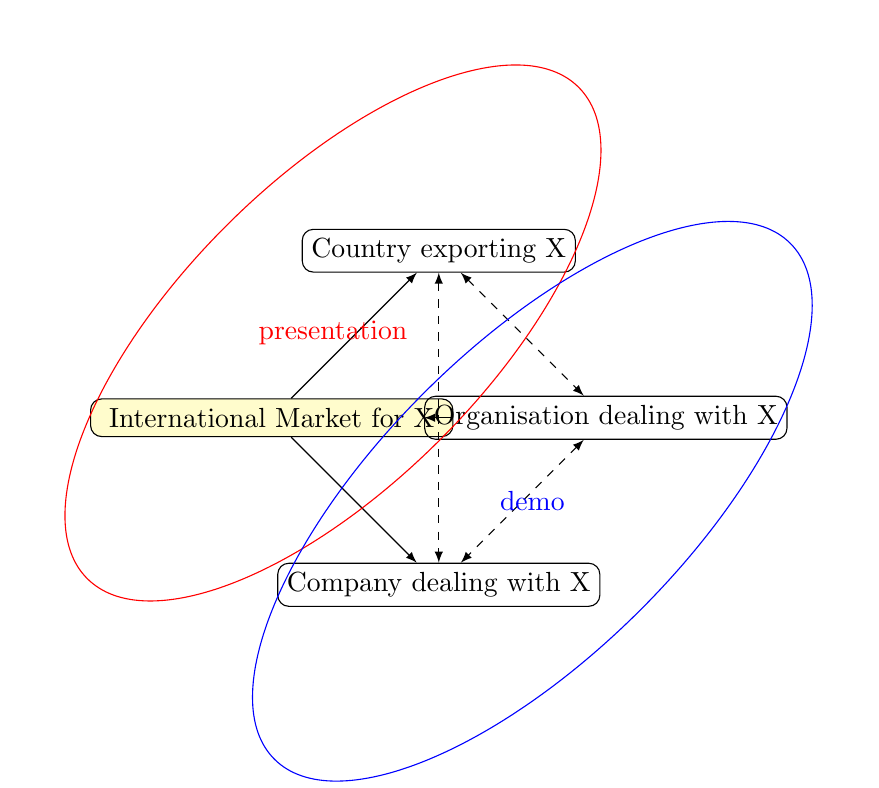
\begin{tikzpicture}[rotate=-45]
    \node[draw, rounded corners,fill=yellow!20] (market) at (0,0) {\mynodebox{
        International Market for X
    }
    };
    \node[draw, rounded corners] (country) at (0,3) {\mynodebox{Country exporting X}};

    \draw[->, >=latex] (market) -- (country);

    

        \node[draw, rounded corners] (company) at (3,0) {\mynodebox{Company dealing with X}};
        \node[draw, rounded corners] (organisation) at (3,3) {\mynodebox{Organisation dealing with X}};
        \draw[<->,>=latex,dashed] (organisation) -- (company);
        \draw[->, >=latex] (market) -- (organisation);
        \draw[->, >=latex] (market) -- (company);
        \draw[<->,>=latex,dashed] (country) -- (organisation);
        \draw[<->,>=latex,dashed] (country) -- (company);

    \ifstep{2}{
\begin{scope}[color=red]

        \node[draw, ellipse, fit=(country) (market), inner sep=1pt,rotate=45] (pr) {};
        \node at (pr) {presentation};
    \end{scope}
}


    \ifstep{3}{
\begin{scope}[color=blue]

        \node[draw, ellipse, fit=(organisation) (company), inner sep=1pt,rotate=45] (pr) {};
        \node at (pr) {demo};
    \end{scope}
}


    
    
\end{tikzpicture}
\end{document}